\chapter{Implementation}
\label{Chapter5}
\lhead{Chapter 5. \emph{Implementation}}

\begin{center}
\rule{0.5\textwidth}{0.5pt}
\end{center}

This chapter presents the implementation of the doc2conv library, an agentic system for generating synthetic conversations for tobacco cessation model training. The library addresses the critical challenge of obtaining high-quality, domain-specific training data through a multi-agent architecture and integration with multiple LLM providers.

\section{System Architecture}

\begin{figure}[h]
    \centering
    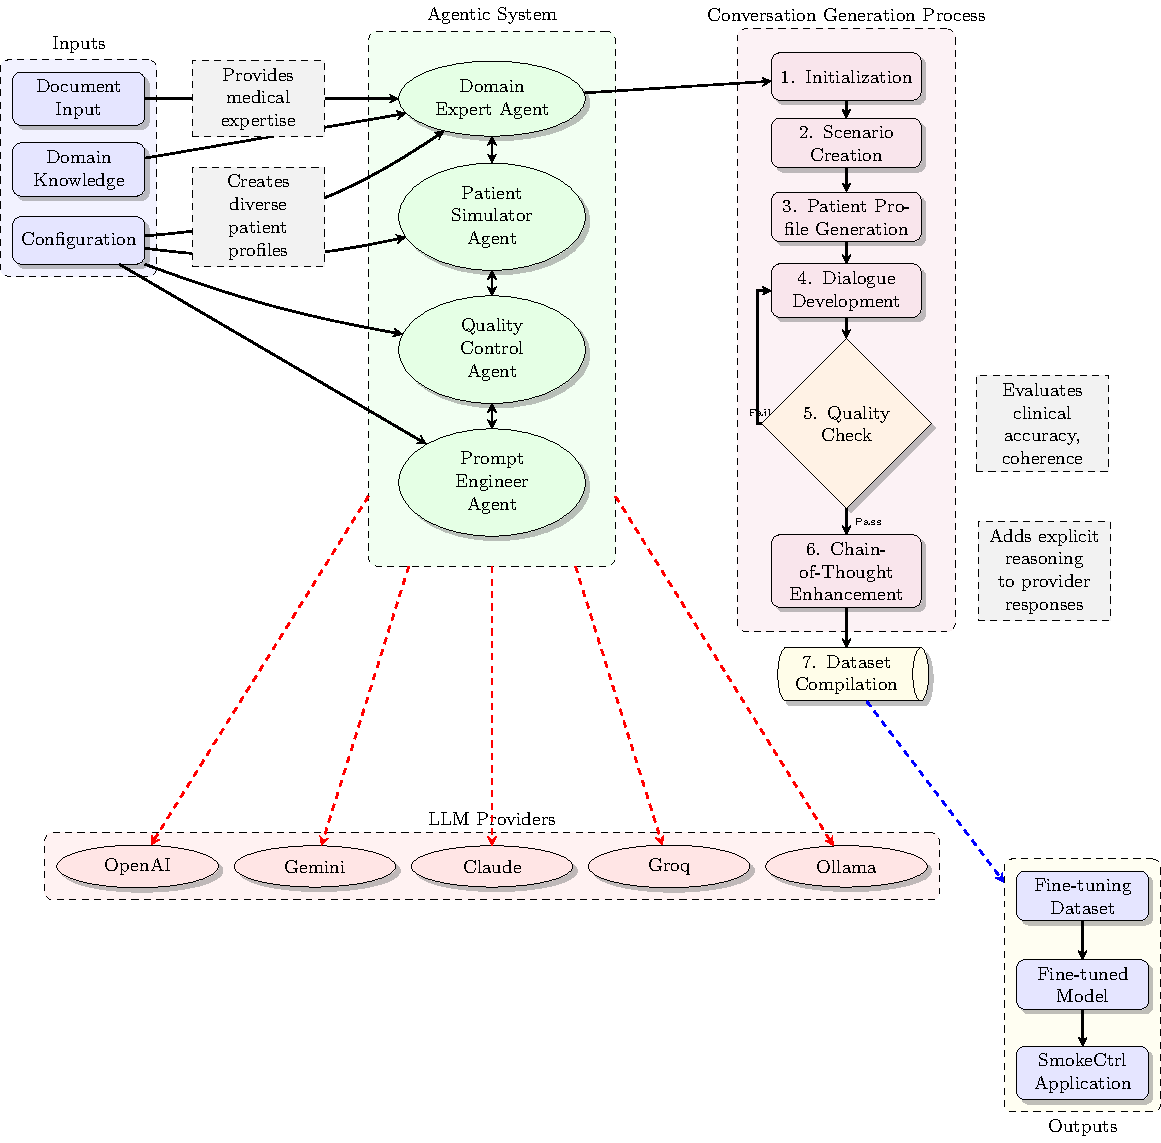
\includegraphics[width=0.85\textwidth]{Pictures/doc2conv_architecture.pdf}
    \caption{Architecture of the doc2conv library showing main components and interactions}
    \label{fig:doc2conv_architecture}
\end{figure}

The doc2conv library transforms static document content into dynamic, interactive conversations through a modular architecture with four primary components:

\begin{itemize}
    \item \textbf{Document Processing}: Extracts and prepares content from various source formats (PDF, DOCX, TXT) while preserving semantic coherence
    
    \item \textbf{Agentic System}: Coordinates specialized agents that collaborate to generate realistic conversations
    
    \item \textbf{LLM Provider Integration}: Connects with multiple LLM services through a consistent interface
    
    \item \textbf{Fine-tuning Preparation}: Formats generated conversations for model training
\end{itemize}

\section{Multi-Agent Implementation}

The system employs four specialized agents, each inheriting from a common \texttt{BaseAgent} class:

\begin{itemize}
    \item \textbf{DomainExpertAgent}: Provides evidence-based tobacco cessation information and ensures clinical accuracy
    
    \item \textbf{PatientSimulatorAgent}: Creates diverse patient profiles and generates realistic responses based on demographic characteristics and tobacco use patterns
    
    \item \textbf{QualityControlAgent}: Evaluates conversations for coherence, relevance, and adherence to healthcare communication standards
    
    \item \textbf{PromptEngineerAgent}: Designs effective prompts for conversation generation, including scenario creation and chain-of-thought templates
\end{itemize}

The \texttt{BaseAgent} class provides common functionality for LLM integration, chain-of-thought support, logging, and error handling. Each agent implements a \texttt{run} method that takes a task description and context as input and returns the agent's specialized output.

\section{LLM Provider Integration}

The library integrates with multiple LLM providers through a provider-specific adapter pattern:

\begin{itemize}
    \item \textbf{Supported Providers}: OpenAI, Google Gemini, Anthropic Claude, Groq, and Ollama
    
    \item \textbf{Common Interface}: Each provider client implements standardized methods for chat completion, embedding generation, and streaming responses
    
    \item \textbf{Provider Selection}: Implements capability-based routing, cost optimization, and performance benchmarking for optimal provider selection
    
    \item \textbf{Error Handling}: Includes robust error recovery, rate limiting, and retry logic for reliable operation
\end{itemize}

\section{Conversation Generation Process}

\begin{figure}[h]
    \centering
    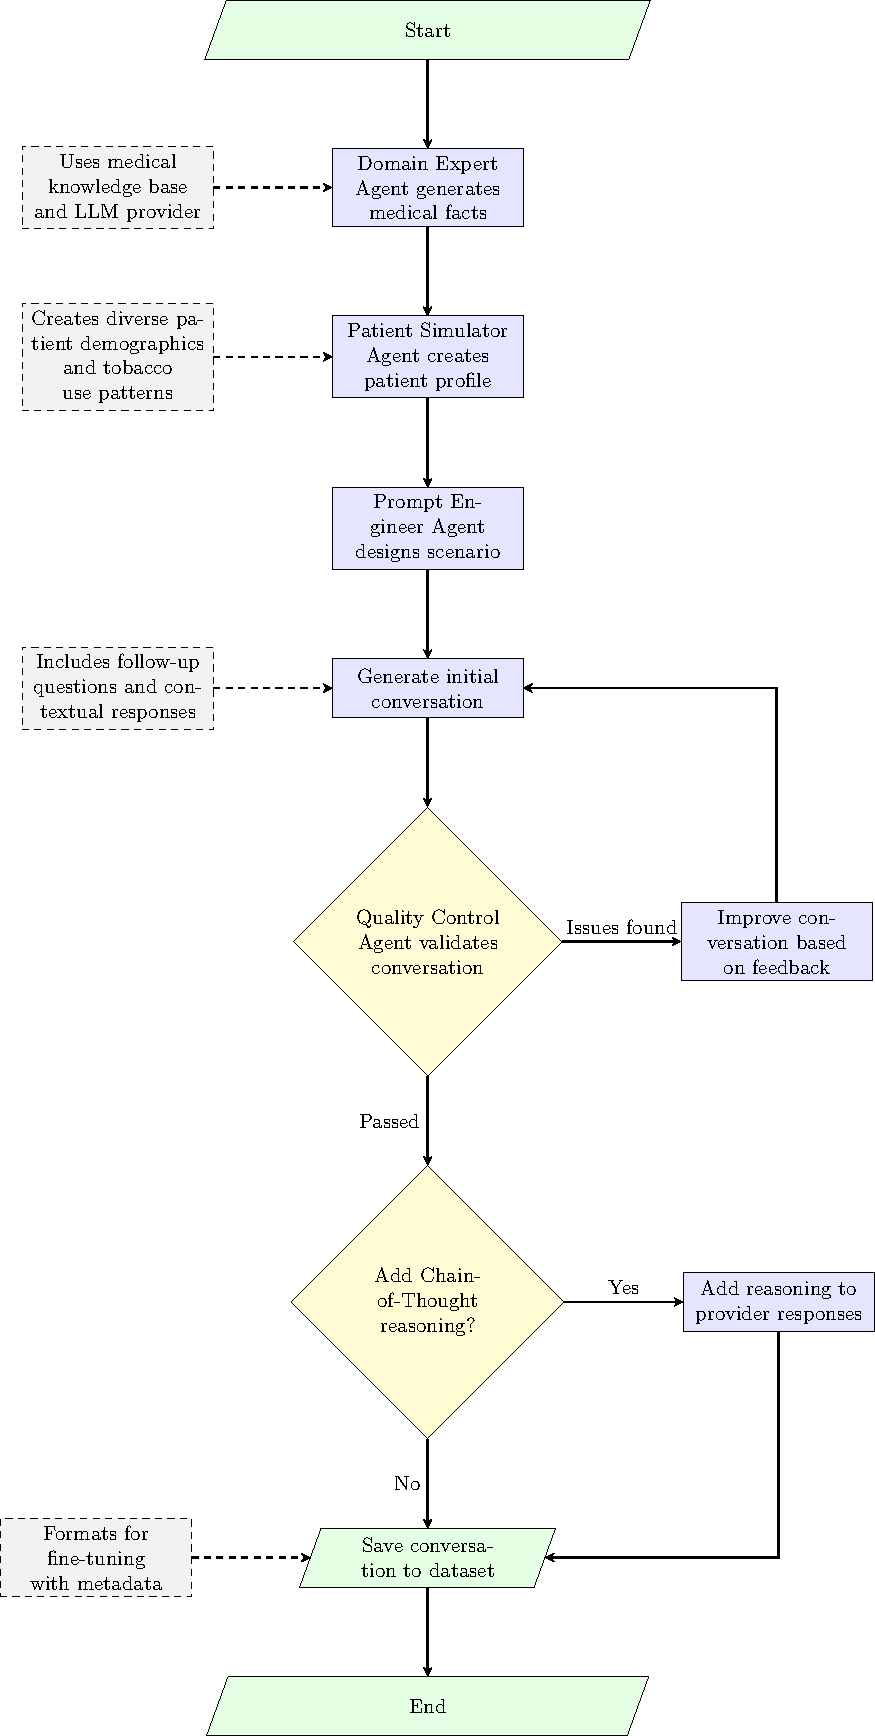
\includegraphics[width=0.75\textwidth]{Pictures/conversation_generation_flow.pdf}
    \caption{Flowchart of the conversation generation process}
    \label{fig:conversation_flow}
\end{figure}

The conversation generation process follows a structured workflow:

\begin{enumerate}
    \item \textbf{Initialization}: Configure agents and LLM providers based on parameters
    
    \item \textbf{Scenario Creation}: Generate context-specific prompts for different conversation types
    
    \item \textbf{Patient Profile Generation}: Create diverse patient characteristics and tobacco use patterns
    
    \item \textbf{Dialogue Development}: Generate multi-turn conversations with agent contributions
    
    \item \textbf{Quality Validation}: Review for factual accuracy, coherence, and adherence to standards
    
    \item \textbf{Chain-of-Thought Enhancement}: Add explicit reasoning processes to healthcare provider responses
    
    \item \textbf{Dataset Compilation}: Format validated conversations for model fine-tuning
\end{enumerate}

\section{Chain-of-Thought Implementation}

A key innovation in doc2conv is the integration of chain-of-thought (CoT) reasoning, which enhances transparency and quality of generated healthcare advice:

\begin{itemize}
    \item \textbf{CoT Prompt Templates}: Specialized prompts that elicit step-by-step reasoning
    
    \item \textbf{Reasoning Generation}: Explicit documentation of assessment, medical facts, and justification for each response
    
    \item \textbf{Response-Reasoning Pairing}: Association of each response with its corresponding reasoning process
    
    \item \textbf{Format Standardization}: Consistent formatting across different LLM providers
\end{itemize}

This approach improves model training by providing explicit reasoning processes that enhance transparency, accuracy, and educational value of the generated conversations.

\section{Module Structure}

The library is implemented as a modular Python package with clear separation of concerns:

\begin{itemize}
    \item \textbf{agents}: Contains implementations of specialized agents
    
    \item \textbf{models}: Provides adapters for different LLM providers
    
    \item \textbf{conversation}: Implements generation, validation, and diversity mechanisms
    
    \item \textbf{finetune}: Handles dataset preparation and training configuration
\end{itemize}

The implementation follows object-oriented design principles with abstract base classes, dependency injection, and comprehensive configuration management to ensure flexibility and maintainability.
